\documentclass[12pt]{article}
\usepackage{fullpage,geometry,amsmath,hyperref,graphicx,xcolor,amssymb,array}
\usepackage{indentfirst}
\newcommand\norm[1]{\left\lVert#1\right\rVert}
\newcommand\normx[1]{\left\Vert#1\right\Vert}
\geometry{letterpaper,left=2.54cm,right=2.54cm,top=2.54cm,bottom=2.54cm}

\begin{document}
\begin{center}\Large\bf 
CS 357 - 15 Solving Nonlinear Equations\\
\end{center}
\begin{center}
Boyang Li (boyangl3)
\end{center}

\medskip

\noindent \textbf{Root of a function: }For a function $f(x) : \mathbb{R} \to \mathbb{R}$, the root of a function is all $x \in \mathbb{R}$ such that $f(x) = 0$. For a multi-dimensional function, the root is all vector $\mathbf{x}$ in the domain such that $f(\mathbf{x}) = \vec{0}$.

\medskip
\noindent \textbf{Solution of an Equation: }For an equation $f(x) = y$, we can construct a new function such that $\tilde{f}(x) = f(x) - y$m then the roots of $\tilde{f}(x)$ are the solutions of $f(x)=y$. This applies to multi-dimensional equations as well.

\medskip
\noindent \textbf{General Methods: }Sometimes it is not easy to apply theorems to some nonlinear equations, so we need to approximate the solution. The basic logistic is ``Initial Guess - Check Residual - Iteration".

\medskip
\noindent \textbf{Convergence: }Iterative methods converges with rate $r$ if
$$\lim_{k \to \infty} \frac{\norm{e_{k+1}}}{\norm{e_k}^r} = C$$
where $e_i$ is the error at iteration $i$, and $C$ is a constant.

The speed of convergence is determined by the value of $r$:
\begin{center}
        \begin{tabular}{ | c | c | c | } 
              \hline
              $\mathbf{r}$ & \textbf{Type of convergence} & \textbf{Accurate digits} \\ 
              \hline
              1 & Linear & Gain constant accurate digits every iteration \\ 
              \hline
              1 < $r$ < 2 & Superlinear & \\ 
              \hline
              2 & Quadratic & Double the number of accurate digits every iteration \\ 
              \hline
        \end{tabular}
    \end{center}

\medskip
\noindent \textbf{Bisection Method: }
\begin{itemize}

\item \textbf{Iteration Steps:}
    \begin{enumerate}
        \item Take 2 points $a$ and $b$ and make sure $f(a) \cdot f(b) < 0$.
        \item Take the midpoint of $[a, b]$, $c = \dfrac{a+b}{2}$.
        \item Evaluate $f(c)$ and use $c$ to replace either $a$ or $b$, to make the signs of 2 endpoints are still opposite.
    \end{enumerate}
\item \textbf{Convergence:} Linear convergence, $e_k = \dfrac{b-a}{2^k}$ and $C = \dfrac{1}{2}$.
\item \textbf{Cost: }Except the fist iteration, every iteration requires one new function evaluation.
\item \textbf{Drawback:} Applicable to functions that we can get the points $a$ and $b$ such that $f(a)$ and $f(b)$ have opposite signs.
\end{itemize}

\newpage
\noindent \textbf{Newton's Method:}
\begin{itemize}
    \item \textbf{Motivation:} $f(x_k+h_k) \approx f(x_k) + f'(x_k) \cdot h_k$ (First 2 terms of Taylor's expansion)
    \item \textbf{Iteration Steps:}
        \begin{enumerate}
            \item $f(x_k) + f'(x_k)\cdot h_k = 0 \to h_k = -\dfrac{f(x_k)}{f'(x_k)}$ ($h_k$ is called Newton step)
            \item $x_{k+1} = x_k + h_k = x_k - \dfrac{f(x_k)}{f'(x_k)}$ (This step is called Newton update)
        \end{enumerate}
    \item \textbf{Convergence:} Quadratic convergence.
    \item \textbf{Cost:} Each iteration we need to evaluate 2 functions, $f(x_k)$ and $f'(x_k)$.
    \item \textbf{Drawbacks: }
        \begin{itemize}
            \item Cost of computing functions
            \item Requires differentiable functions
            \item Initial guess need to be close to the solution/root, otherwise, it will be divergence.
        \end{itemize}
\end{itemize}

\medskip
\noindent \textbf{Secant Method:} 
\begin{itemize}
    \item \textbf{Relation with Newton's Method:} Sometimes we cannot evaluate the derivative of a function directly, so we need to approximate the derivative by applying
    $$f'(x_k) \approx \frac{f(x_k) - f (x_{k-1})}{x_k - x_{k-1}}$$
    \item \textbf{Iteration Steps: }Same as Newton's Method.
    \item \textbf{Convergence:} Superlinear convergence, $r = \dfrac{\sqrt{5}+1}{2}$.
    \item \textbf{Cost:} Except the first iteration, every iteration requires one function evaluation.
    \item \textbf{Drawbacks:}
        \begin{itemize}
            \item Same as Newton's methods but does not require a derivative
            \item Not converge as quickly as Newton's method
            \item Need 2 initial guesses near the root
        \end{itemize}
\end{itemize}

\newpage
\noindent \textbf{1D Summary (From CS357 Online Textbook):}
    \begin{center}
    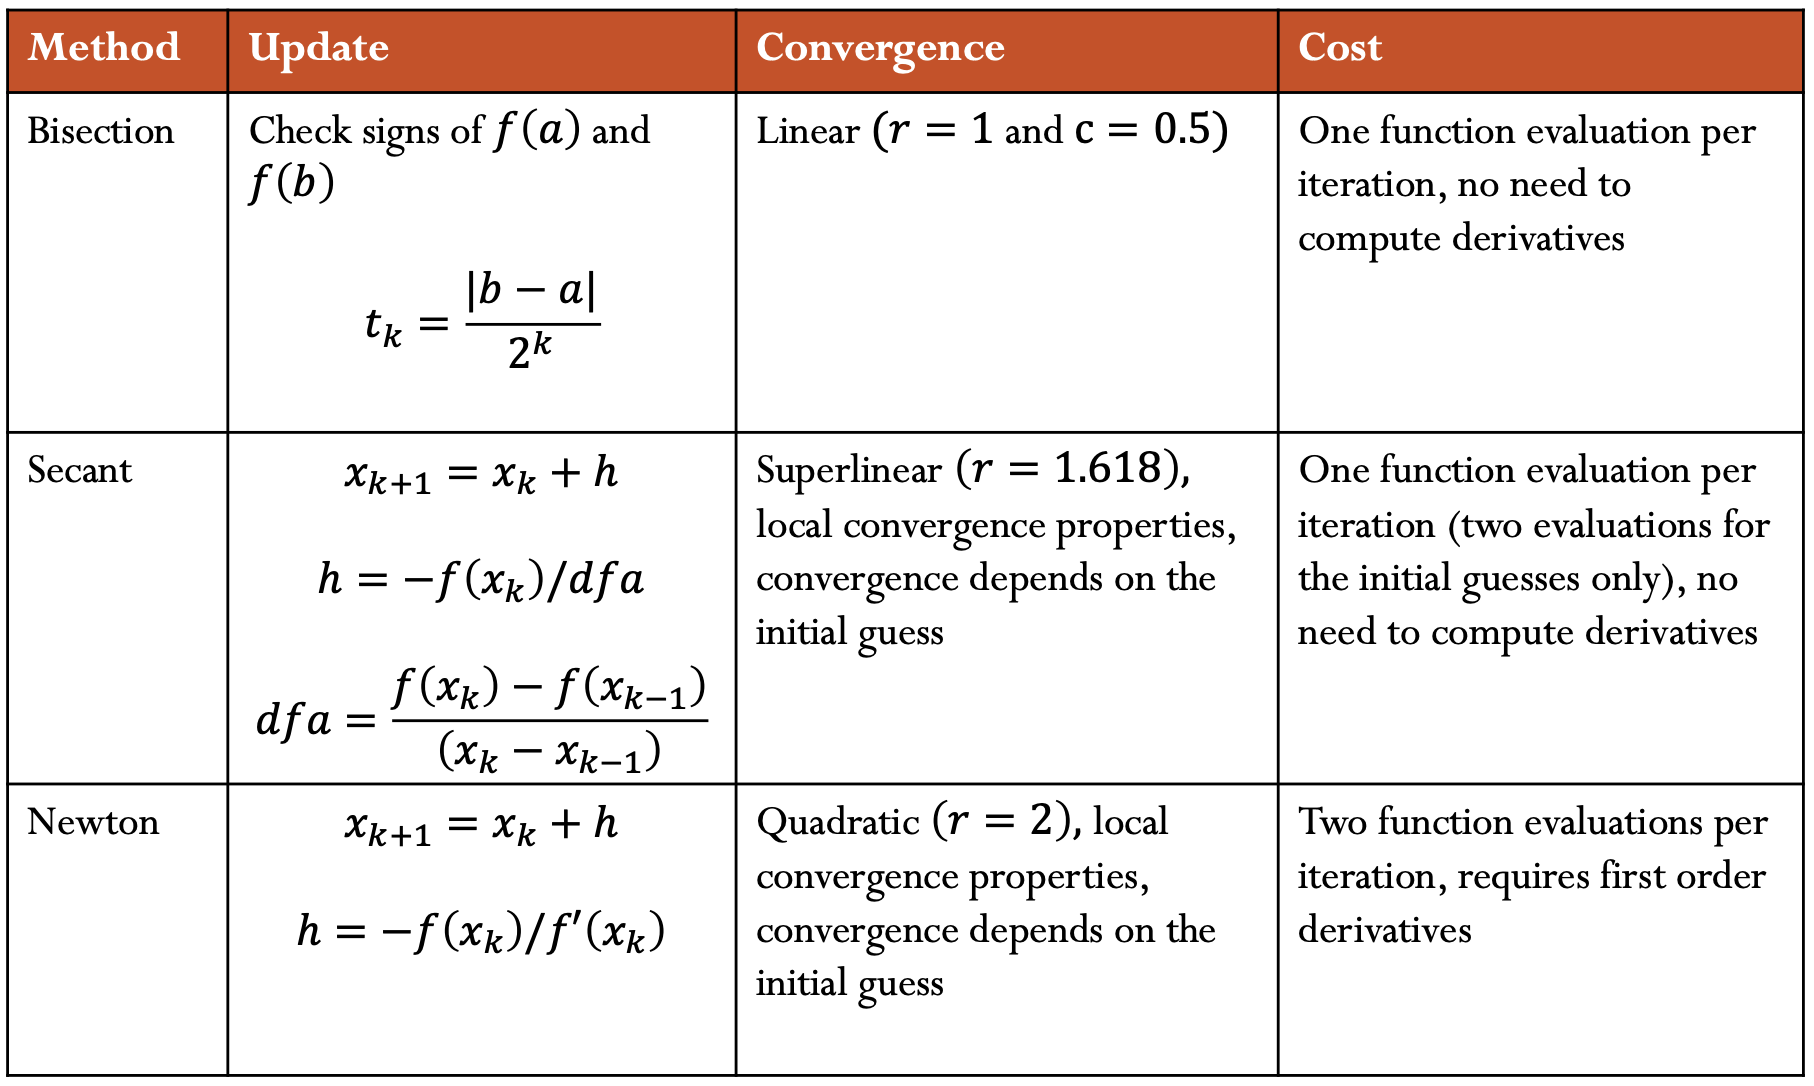
\includegraphics[width= 1\linewidth]{1Dsummaries.png}
    \end{center}

\medskip
\noindent \textbf{N-D Newton's Method: }
\begin{itemize}
    \item \textbf{Motivation:} $f(\mathbf{x}_k + \mathbf{s}_k) \approx f(\mathbf{x}_k) + \mathbb{J}(\mathbf{x}_k) \cdot \mathbf{s}_k$ (Introduced from 1-D Newton's Method, where $\mathbb{J}(\mathbf{x})$ is the Jacobian matrix of $f(\mathbf{x})$.
    \item \textbf{Iteration Steps:}
        \begin{enumerate}
            \item $f(\mathbf{x}_k) + \mathbb{J}(\mathbf{x}_k) \cdot \mathbf{s}_k = 0 \to \mathbf{s}_k = - \mathbb{J}(\mathbf{x}_k)^{-1} \cdot f(\mathbf{x}_k)$ ($\mathbf{s}_k$ can also be calculated by solving the system $\mathbb{J}(\mathbf{x}_k) \cdot \mathbf{s}_k = -f(\mathbf{x}_k)$). 
            \item $\mathbf{x}_{k+1} = \mathbf{x}_k + \mathbf{s}_k = \mathbf{x}_k - \mathbb{J}(\mathbf{x}_k)^{-1} \cdot f(\mathbf{x}_k)$
        \end{enumerate}
    \item \textbf{Cost:} The cost of calculating $\mathbf{s}$ by solving the linear system is $\mathcal{O}(n^3)$, the cost of calculating $\mathbb{J}(\mathbf{x})$ is $\mathcal{O}(n^2)$.
    \item \textbf{Drawbacks:}
        \begin{itemize}
            \item Like 1D, only converges locally
            \item Expensive to compute Jacobian matrix and solve linear system.
        \end{itemize}
\end{itemize}

\end{document}

